

\documentclass{article}

\usepackage[utf8]{inputenc} %% Pour pouvoir utiliser les caractères accentués
\usepackage{graphicx} %% Pour pouvoir inclure des graphiques

\title{{\Huge \bf ENIB 2012 : S2P  MDD} \\
\vspace*{2cm}
{\Huge \bf Medius} \\----\\ Document de conception \\
\vspace*{2cm}
\centerline{
\includegraphics[height=3cm]{logomedius.jpg}}
}
\author{Valérian Saliou (v1saliou) \& Kwon-Young Choi (k1choi)}

%\date{La date}
\date\today 

\begin{document}
\maketitle

\newpage

\section{Rappel des versions}

\subsection{Version 1 : accéder au menu}
\begin{itemize}
\item afficher le fond animé (2 couches)
\item configurer le son (effets et musique)
\end{itemize}

\subsection{Version 2 : accéder aux niveaux}
\begin{itemize}
\item afficher les niveaux
\item lancer un niveau
\item obtenir des détails sur un niveau (document d'aide)
\end{itemize}

\subsection{Version 3 : accéder aux combats \#1}
\begin{itemize}
\item combattre une bactérie
\item afficher les organismes ennemis
\item gérer les tirs
\item gérer les vies
\item gérer les collisions
\item gérer la vitesse
\end{itemize}

\subsection{Version 4 : accéder aux combats \#2}
\begin{itemize}
\item combattre un virus
\item gérer les maladies (1 scénario par maladie, virus ou bactérie)
\end{itemize}
\newpage

\section{Analyse nom-verbe}

\begin{itemize}
\item Fond de menu
  \begin{itemize}
  \item afficher
  \end{itemize}
\item Boutons
  \begin{itemize}
  \item afficher
  \item créer handlers de clic
  \end{itemize}
\item Jeu
  \begin{itemize}
  \item accéder à la liste des niveaux
  \end{itemize}
\item Configuration
  \begin{itemize}
  \item afficher les checkboxes
  \item callback au changement de valeur
  \end{itemize}
\end{itemize}

\newpage
\section{Définition des types de données}

\begin{verbatim}

type menu = struct
             background : Background
             decor : Decor
             bouton : Bouton
             checkbox : Checkedbox
             fstruct				

type Background = struct
             sprite : Sprite
             speed : Vec
             fstruct

type Decor = struct
             spriteTop : Sprite
             spriteBottom : Sprite
             spriteLogo : Sprite
             true : Bool
             fstruct

type Bouton = struct
             sprite : Sprite
             target : Function
             true : Bool
             fstruct

type Checkedbox= struct
             sprite.uncheck : Sprite
             sprite.check : Sprite
             target : Sound
             check : Bool
             true : Bool
             fstruct

type Game :
             background : Background
             bacteria : Bacteria
             phagocyte : Phagocyte

type Bacteria =struct
             sprite : Sprite
             speed : Vec
             animation.attaque : Anim
             animation.duplication : Anim
             animation.destruction : Anim
             fstruct
type Phagocyte =struct
             sprite : Sprite
             speed : Vec
             animation.attaque : Anim
             animation.destruction : Anim

Sprite = struct
             image : Image
             position : Vec
             size : Vec
             fstruct

Vec = struct
             a : int
             b : int
             fstruct

Anim = struct
             image1 : Image
             image2 : Image
             image3 : Image
             image4 : Image
             image5 : Image
             position : Vec
             fstruct

Function = struct
             module : Text
             function : Text
             fstruct

Sound = struct
             pathSound1 : Text
             pathSound2 : Text
             pathSound3 : Text
             pathSound4 : Text
             lengthSound1 : float
             lengthSound2 : float
             lengthSound3 : float
             lengthSound4 : float
             fstruct

\end{verbatim}
\newpage
\section{Modules}

\begin{tabular}{||l|l||}
 \hline main.py : initialisation et définition des fonctions callback. \\
 \hline menu.py : gère le menu \\
 \hline background.py : gère le fond d'écran \\
 \hline decor.py : gère le décor \\
 \hline button.py : gère les boutons dans le menu \\
 \hline checkbox.py : gère les checkbox du menu \\
 \hline game.py : gère les appels de fonction pour le jeu \\
 \hline bacteria.py : gère les bactéries \\
 \hline phagocyte.py : gère le héros \\
 \hline sprite.py : gère les sprites \\
 \hline vec.py : gère les vecteurs \\
 \hline anim.py : gère les animations \\
 \hline function.py : gère les fonctions cibles des boutons \\
 \hline sound.py : gère les sons \\
 \hline
\end{tabular}
\newpage

\section{Arbre des appels de fonctions}

\subsection{Initialisation}

\begin{center}
\begin{figure}[h]
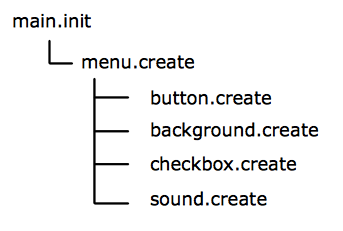
\includegraphics[scale=0.5]{arbre_init.png}
\end{figure}
\end{center}

\subsection{Affichage}
\begin{center}
\begin{figure}[h]
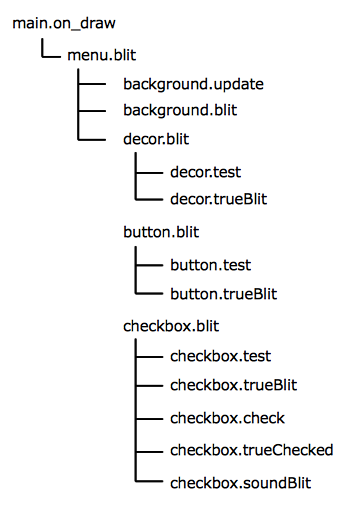
\includegraphics[scale=0.5]{arbre_ondraw.png}
\end{figure}
\end{center}
\newpage
\section{Description synthétique des fonctions}

\begin{verbatim}
main.init :
             enchaine les fonctions d'initialisation

menu.create :
             enchaine les fonctions d'initialisation

levels.create :
             lister les niveaux

levels.help :
             obtenir de l'aide sur un niveau

game.create :
             créer un jeu

background.create :
             crée en mémoire une représentation du fond d'écran (image + position + speed)

decor.create :
             crée en mémoire une représentation du décor (images + position)

button.create :
             crée en mémoire une représentation d'un boutton (image + position + size + target + true)

checkbox.create :
             crée en mémoire une représentation d'un checkbox (images + position + size + target + check + true)

sound.create :
             crée en mémoire une représentation du son

main.on_draw :
             affiche l'image, appelé régulièrement par Pyglet

menu.blit :
             enchaine les fonctions qui crée les représentations graphiques des différents objets qui constituent le menu.

background.update :
             met à jour la position du fond d'écran

background.blit :
             affiche le fond d'écran

decor.blit :
             affiche le décor que si cela est requis.

decor.test :
             test si le décor doit être afficher ou non. 
             Renvoie True si le décor doit être visible, False sinon

decor.trueBlit :
             affiche le décor

button.blit :
             affiche le bouton que si cela est requis.

button.test :
             test si le bouton doit être afficher ou non.
             Renvoie True si le bouton doit être visible, False sinon

button.trueBlit :
             affiche le bouton

checkbox.blit :
             affiche le checkbox que si cela est requis et en fonction de son état checké ou non.

checkbox.test :
             test si le checkbox doit être afficher ou non.
             Renvoie True si le checkbox doit être visible, False sinon

checkbox.trueBlit :
             affiche le checkbox non checké

checkbox.check :
             test si le checkbox est checké ou non.   
             Renvoie True si le checkbox doit être visible et checké, False sinon

checkbox.trueChecked :
             affiche le checkbox checké

main.on_mouse_press :
             gère les cliques de souris, appelée régulièrement.

menu.mousePressEvent :
             enchaine les fonction lors d'un clic de souris.

menu.mousePosition :
             récupère la position de la souris lors d'un clic et l'envoie aux fonctions concernées.

button.mousePressCheck :
             vérifie et renvoie True si le clic de la souris s'est effectué sur le bouton, False sinon.

button.target :
             appelle la fonction cible du bouton (par exemple la fonction game pour le bouton jeu)

checkbox.mousePressCheck :
             vérifie si le clic s'est effectué sur la checkbox et marque si la checkbox est checké ou non. Renvoie True si la checkbox à été checké, False sinon.

checkbox.target :
             appelle la  cible de la checkbox (par exemple de la musique)

\end{verbatim}

 

\newpage
\section{Calendrier de développement}
Notre développement est progressif. Dans un premier temps nous nous concentrons sur un menu propre et complètement fonctionnel, de même pour le sélecteur de niveaux. Seulement ensuite, nous développerons les niveaux avec la gestion des combats.\\
	
Il s'agit de poser des bases de travail dans un premier temps, nous permettant de disposer d'un environnement de jeu paramétrable sur lequel les niveaux viennent se greffer.

\begin{itemize}
\item Mars 2012 : 
  \begin{itemize}
  \item Création de \begin{tt}menu.create\end{tt} 
  \item Création de \begin{tt}background.create\end{tt}
  \item Création de \begin{tt}button.create\end{tt}
  \item Création de \begin{tt}checkbox.create\end{tt}
  \end{itemize}

\item Avril 2012 : 
  \begin{itemize}
  \item Création de \begin{tt}levels.create\end{tt}
  \item Création de \begin{tt}levels.help\end{tt}
  \item Création de \begin{tt}game.create\end{tt}
  \end{itemize}


\item Mai 2012 (1ère moitié) : 
  \begin{itemize}
  \item Création de \begin{tt}bacteria.add\end{tt}
  \end{itemize}

\item Mai 2012 (2nde moitié) :
  \begin{itemize}
  \item Création de \begin{tt}virus.add\end{tt}
  \end{itemize}
\end{itemize}
\newpage
\section{Annexe : Description détaillée des fonctions}

\subsection{Module main.py}

\subsubsection{Fonction init}

\begin{verbatim}
PARAMETRES : 
  aucun

RESULTAT : 
  aucun

ROLE :
  enchaîne les fonctions d'initialisation

PRECONDITIONS : 
  le script est appelé en tant que parent, et non inclus dans un script parent

POSTCONDITIONS :
  la configuration est chargée, le menu est créé, les boutons associés sont ajoutés
\end{verbatim}

\end{document}